% -*-cap1.tex-*-
% Este fichero es parte de la plantilla LaTeX para
% la realización de Proyectos Final de Carrera, protejido
% bajo los términos de la licencia GFDL.
% Para más información, la licencia completa viene incluida en el
% fichero fdl-1.3.tex

% Copyright (C) 2009 Pablo Recio Quijano 

%\section{Introducción}

A continuación se muestran los resultados del estudio tal y como se describieron en la sección anterior.

\section{Localización de la literatura}
En la tabla \ref{tab:ResumenBusquedaResultados} se muestran las búsquedas realizadas en las bibliotecas digitales más importantes en ciencias de la computación, los términos de búsqueda utilizados y el número de documentos obtenidos. Se realizarion numerosas pruebas de búsqueda, ya que los resultados obtenidos cuando el filtrado era muy riguroso menguaba de manera considerable. Sin embargo, relajar el filtro suponía la proliferación de literatura relacionada muy vagamente con nuestro ámbito de investigación. Esto es así porque en prácticamente todos los ámbitos de la ciencia se está fomentando el desarrollo de competencias genéricas, sin embargo, no todos los estudios abordan su evaluación, y mucho menos lo hacen de manera automizada. Realizar la búsqueda por el término "Assessment of generic skills" o "assessing generic skills" nos planteaba la primera problemática, y es que el número de artículos para devueltos era muy reducido. Sin embargo, debilitando la búsqueda con términos como "generic competences" o "generic skills" junto con la palabra "assessment" daba un número de resultados muy elevado. Por esto, finalmente se optó por añadir a esta segunda casuística nomenclatura relacionada con la evalación asistida por ordenador: TEL (Technology Enhanced Learning), ICT (Information and communications technology), CBI (computer-based instruction), o LMS (Learning Managment System). En cada biblioteca, se utilizaron los formularios de búsqueda avanzada.

\begin{table}[H]
  \begin{center}
  \begin{tabular}{| m{3.5cm} | m{6cm} | m{3cm} | c |}
    \hline
    SOURCE & SEARCH TERMS & SEARCH SCOPE & RESULTS\\
    \hline
    \hline
    Wiley Online Library & assessment AND ``generic competences`` OR ``generic skills`` AND (TEL OR ICT OR CBI) & in All Fields & 140 \\
    \hline
    World Scientific Net & ``generic competences`` OR ``generic skills`` AND assessment & Anywhere in article & 20\\
    \hline
    Springer & (``generic skills`` OR ``generic competences``) AND  students AND (TEL OR CBI OR ICT) & All fields (Including full text) & 141\\
    \hline
    ACM Digital Library & (assessment and ``generic skills``) and (TEL or LMS or ICT or CBI) & Any field (title, abstract, review) & 57\\
    \hline
    ACM Digital Library & (assessment and ``generic competences``) and (TEL or LMS or ICT or CBI) & Any field (title, abstract, review) & 15\\
    \hline
    IEEE Digital Library (Xplore) & (((TEL or LMS or ICT or CBI) AND (``generic skills`` OR ``generic competences``)) AND assessment) & Full text and metadata & 48\\
    \hline
    Scopus & (((TEL or LMS or ICT or CBI) AND (``generic skills`` OR ``generic competences``)) AND assessment) & All fields (Including full text) & 47\\
    \hline
    \multicolumn{3}{|r|}{TOTAL} & 467\\
    \hline
  \end{tabular}
\end{center}
\caption{Bibliotecas digitales utilizadas, palabras de búsqueda utilizadas en cada uno y número de resultados obtenidos}
\label{tab:ResumenBusquedaResultados}
\end{table} 


%\section{Selección de trabajos}
%En la tabla \ref{tab:ResumenSelecccionResultados} se muestran los resultados de la clasificación.

En total se recopilaron 468 trabajos, que fueron revisados para identificar si eran de utilidad para el estudio y descartados si cumplían alguno de los criterios de exclusión. El número de estudios primarios resultante (después de aplicar criterios de selección y exclusión) fue de sólo 32 trabajos (casi un 7\% del total de trabajos recopilados). Aunque hay muchos trabajos que tratan las competencias genéricas desde diferentes perspectivas, son muy pocos los que abordan su evaluación desde el punto de vista de la tecnología. De ahí estos resultados, cuya primera y optimista interpretación es que pudiera haber un nicho de investigación. Los resultados de esta clasificación pueden verse e la tabla \ref{tab:ResumenSelecccionResultados}.

\begin{table}[H]
  \begin{center}
  \begin{tabular}{| m{4cm} | c | c |}
    \hline
    CRITERION & STUDIES & FRECUENCY\\
    \hline
    \hline 
    Included & 32 & 6,84\% \\
    \hline
    Off Topic & 407 & 86,97\% \\
    \hline
    Unsupported Language & 1 & 0,21\% \\
    \hline
    Duplicated & 20 & 4,27\% \\
    \hline
    Unread & 8 & 1,71\% \\
    \hline
    Total & 468 & 100\% \\
    \hline
  \end{tabular}
\end{center}
\caption{Clasificación de trabajos una vez aplicados los criterios de selección y exclusión}
\label{tab:ResumenSelecccionResultados}
\end{table} 


%\section{Extracción de los datos}
%Se han seleccionado como estudio primario únicamente 37 artículos, un 7,92\% del total de los revisados. Casi la mayor parte de los seleccionados se pueden localizar en los últimos años, entre 2008 y 2013 (Tabla \ref{tab:ResumenAniosResultados} y figura \ref{fig:PublicacionesAnuales}). 

Aunque hace varios años desde que las tecnologías entraron a formar parte de la vida académica, no es hasta 2010, con lo que la Comisión Europea llama la tercera generación de herramientas, cuando se comienzan a integrar la evaluación en las herramientas de aprendizaje, y conceptos como "Data Mining and analysis", "Behavioural tracking" and "Learning analytics" comienzan a asomar \cite{Redecker:2013}. Con esta introducción, damos sentido a la distribución de la producción de la selección primaria a lo largo de los años, que puede verse tanto en la tabla \ref{tab:ResumenAniosResultados} como en la figura \ref{fig:PublicacionesAnuales}. Casi la mayor parte de los seleccionados se pueden localizar en los últimos años, entre 2011 y 2013.


\begin{table}[H]
  \begin{center}
  \begin{tabular}{| m{4cm} | c |}
    \hline
    YEAR & RESULTS\\
    \hline    
    \hline
    2003 & 0\\
    \hline
    2004 & 0\\
    \hline
    2005 & 0\\
    \hline
    2006 & 2\\
    \hline
    2007 & 1\\
    \hline
    2008 & 6\\
    \hline
    2009 & 1\\
    \hline
    2010 & 2\\
    \hline
    2011 & 5\\
    \hline
    2012 & 5\\
    \hline
    2013 & 10 \\
    \hline
  \end{tabular}
\end{center}
\caption{Cantidad de trabajos publicados cada año}
\label{tab:ResumenAniosResultados}
\end{table} 

\begin{figure}[H]
  \begin{center}
    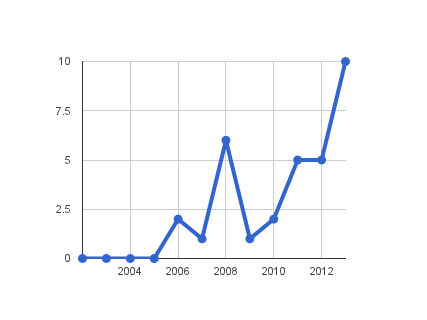
\includegraphics[scale=0.7]{cap3_pub_anuales.png}
  \end{center}
  \caption{Distribución de las publicaciones por años}
  \label{fig:PublicacionesAnuales}
\end{figure}

La revista es el medio en el que más de este tipo de artículos se han publicado, tal y como se puede consultar en la tabla \ref{tab:ResumenForumResultados} y en la figura \ref{fig:PublicacionesTipos} con un 53,1\% del total. Esta información se complementa con la distribución de las publicaciones según el foro en el que han sido publicados y que se muestra en la tabla \ref{tab:DistribucionPublicaciones}. En este se puede comprobar como la mayor parte de las publicaciones están relacionadas con la ingeniería y la educación: World Scientific and Engineering Academy and Society Conferences (WSEAS), IEEE Global Engineering Education Conference (EDUCON), European Journal of Education o Revista Iberoamericana de Tecnologías del Aprendizaje (RITA), entre otras, son las publicaciones que más trabajos han aportado a nuestro trabajo.

\begin{table}[H]
  \begin{center}
  \begin{tabular}{| m{4cm} | c |}
    \hline
    PUBLICATION TYPE & RESULTS\\
    \hline
    \hline 
    Journal & 17 \\
    \hline
    Conference & 10 \\
    \hline
    Chapter & 5 \\
    \hline
  \end{tabular}
\end{center}
\caption{Cantidad de trabajos según el medio en el que fueron publicados}
\label{tab:ResumenForumResultados}
\end{table} 

\begin{figure}[H]
  \begin{center}
    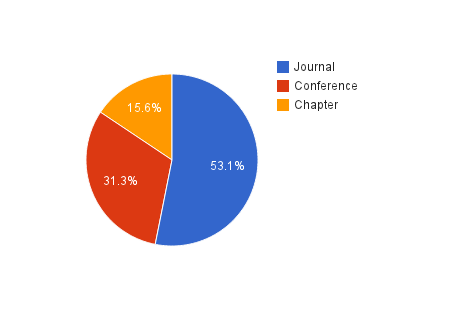
\includegraphics[scale=0.7]{cap3_pub_types.png}
  \end{center}
  \caption{Distribución de publicaciones según el medio en el que fueron publicados}
  \label{fig:PublicacionesTipos}
\end{figure}

\begin{table}[H]
  \begin{center}
  \begin{tabular}{| m{12cm} | c |}
    \hline
    PUBLICATION FORUM & PAPERS\\
    \hline
    \hline 
    World Scientific and Engineering Academy and Society Conferences & 4\\
    \hline
    IEEE Global Engineering Education Conference & 2\\
    \hline
    Australian Society for Computers in Learning in Tertiary Education & 2\\
    \hline
    European Journal of Education & 2\\
    \hline
    Revista Iberoamericana de Tecnologías del Aprendizaje & 2\\
    \hline
    Assessment \& Evaluation in Higher Education & 1\\
    \hline
    Australasian Journal of Educational Technology & 1\\
    \hline
    Conference on Software Engineering Education and Training & 1\\
    \hline
    Competency-based Language Teaching in Higher Education & 1\\
    \hline
    Computers in Human Behavior & 1\\
    \hline
    Computing Colombian Conference & 1\\
    \hline
    Decision Support Systems & 1\\
    \hline
    Game-based learning in higher education and lifelong learning: bridging the gap between theory and practice & 1\\
    \hline
    Human Factors and Ergonomics in Manufacturing \& Service Industries & 1\\
    \hline
    International Conference on Advanced Learning Technologies & 1\\
    \hline
    International Journal of Learning Technology & 1\\
    \hline
    Journal of Computer Assisted Learning & 1\\
    \hline
    Medical Education & 1\\
    \hline
    Revista de Educación & 1\\
    \hline
    The Internet and Higher Education & 1\\
    \hline
    Ubiquitous and Mobile Learning in the Digital Age & 1 \\
    \hline
  \end{tabular}
\end{center}
\caption{Distribución de las publicaciones}
\label{tab:DistribucionPublicaciones}
\end{table} 



\section{Esquema de clasificación y mapeo del estudio}

Una vez revisados todos los artículos se han extraído unas características o categorías comunes a la tipología de los trabajos. Todos los trabajos seleccionados hacen uso de algún tipo de software o metodología para evaluar algún tipo de competencia genérica. Pero ningún trabajo utiliza un enfoque como el que se propone en la introducción de este capítulo, es decir, aprovechando los registros de interacción de los estudiantes con el LMS como indicadores del desempeño de las competencias genéricas. Encontramos trabajos que se apoyan en la tecnología para las competencias pero que terminan delegando parte de la evaluación en el alumno, ya sea mediante autoevaluación o evaluación entre iguales. Otros trabajos se basan en videojuegos o en las redes sociales para evaluar alguna competencia, mientras que otros desarrollan algún tipo de software o técnica. Finalmente hay algunos trabajos que simplemente detectan en su entorno la necesidad de la evaluación de las competencias de manera automática porque su forma de hacerlo les ocasiona una serie de problemas o desventajas con respecto a otro método que proponen o demandan. Además se han encontrado algunas revisiones sobre la literatura relacionadas que también serán tratadas a parte.  En la tabla \ref{tab:PublicacionesForum} se puede ver la distribución de las publicaciones, apoyadas gráficamente en la figura  \ref{fig:PublicacionesForum}.

\begin{table}[H]
  \begin{center}
  \begin{tabular}{| m{4cm} | c |}
    \hline
    PUBLICATION ISSUE & PAPERS\\
    \hline
    \hline 
    Evaluaciones & 11\\
    \hline
    Necesidad & 8\\
    \hline
    Red social & 2\\
    \hline
    Videojuegos & 5\\
    \hline
    Revisiones & 3\\
    \hline
    Técnicas & 8 \\
    \hline
  \end{tabular}
\end{center}
\caption{Distribución de publicaciones por tratamiento del problema}
\label{tab:PublicacionesForum}
\end{table} 

\begin{figure}[H]
  \begin{center}
    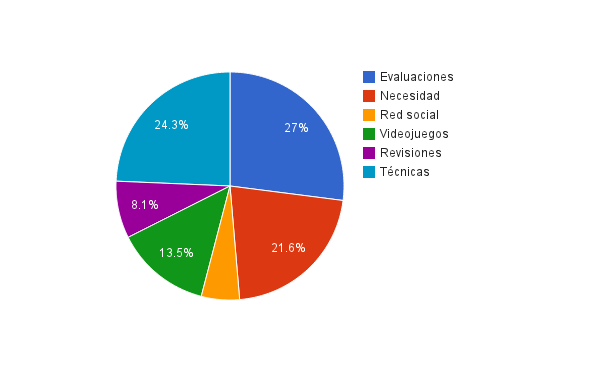
\includegraphics[scale=0.7]{cap3_pub_forum.png}
  \end{center}
  \caption{Distribución de publicaciones por tratamiento del problema}
  \label{fig:PublicacionesForum}
\end{figure}

% Incluir burbujas

\section{Esquema de clasificación}

% Lo dejo aquí. Traer a este esquema de clasificación el reserch scope que puse en el apartado anterior, y en el apartado anterior fijarme en lo que hizo Iván. (Dice algo de step keyworking ...).



En los siguientes apartados, se presentan los resultados del estudio para cada área de investigación. %Los documentos base de este estudio están incluidos en el Apéndice.

\subsection{Metodologías que delegan en los alumnos}
Para favorecer el desarrollo del aprendizaje se utilizan estrategias evaluativas como la autoevaluación, la evaluación entre iguales y la coevaluación. Estas aportan beneficios a estudiantes y profesores universitarios, como la mejora de los procesos y productos del aprendizaje, el desarrollo de estrategias interpersonales, la mejora de la capacidad para emitir juicios o el desarrollo de determinadas competencias académicas y profesionales \cite{Ibarra:2012}. Además, cuando el número de alumnos y la cantidad de información a tener en cuenta en la evaluación crecen, evaluar el trabajo de cada estudiante se vuelve un trabajo muy poco escalable \cite{Balderas:2012}.

Esta estrategia se apoya en el uso de algún tipo de tecnología para trabajar y evaluar una competencia genérica, dejando a posteriori a criterio del alumno la labor de valorar si un compañero o él mismo han alcanzado dicha competencia gracias a la actividad desarrollada. Aunque este enfoque tiene sus beneficios tanto para profesores como para estudiantes, una revisión del profesor podría ser igualmente un trabajo inabarcable.

\subsection{Videojuegos}
Son numerosos los estudios que han tratado las ventajas del aprendizaje basado en juegos (GBL, Game-based learning) \cite{Costu:2009,Munoz:2011}. En estos trabajos se presentan juegos de simulación virtual para cursos que fomentan la colaboración de la universidad y la industria. Juegos que simulan situaciones de la vida real para el desempeño de ciertas competencias y que serán útiles para la industria. Las simulaciones son ambientes de aprendizaje complejos y desafiantes que presentan dificultades para los estudiantes, ya que éstos carecen de una comprensión fundamental de los conceptos específicos del dominio, las relaciones y estrategias de resolución de problemas \cite{Kirkley:2004}. Uno de los factores importantes de esta simulación es la configuración de aprendizaje \cite{Thavikulwat:2010}, la alineación de objetivos, los métodos de aprendizaje y evaluación con los resultados de aprendizaje previstos. Esta evaluación es el aspecto que más nos interesa analizar. Aunque no siempre se realiza de manera automática, sino que a menudo se apoya en el uso de algún tipo de rúbrica facilitada por el LMS.
 
\subsection{Técnicas}
En esta categoría se recogen todos aquellos trabajos que aporten propuestas automáticas o semiautomáticas para la evaluación de competencias genéricas basados en algún modelo. Son herramientas que permiten a los estudiantes, en primer lugar, identificar sus puntos fuertes y débiles y desarrollar estrategias personales para la mejora. En segundo lugar, proporciona a los profesores con información adicional sobre los efectos de su enseñanza en las competencias de los estudiantes. Y por último, proporciona información útil para gestión de la calidad de los programas de enseñanza, ya que puede detectar tendencias en las necesidades de formación de los nuevos estudiantes y ayudar a mejorar el contenido \cite{Achcaoucaou:2012}.

\subsection{Necesidades}
La búsqueda de trabajos relacionados no ha proporcionado muchos resultados directamente relacionados. Sin embargo, aunque no aporten una herramienta concreta, sí hemos encontrado trabajos que detectaban la necesidad de un método, herramienta o modelo para la evaluación de competencias genéricas. Se han añadido a este trabajo los más relevantes de dichos artículos. Este cambio conceptual en el área de la evaluación asistida tiene su motivación en el cambio pedagógico global de conocimiento para el aprendizaje basado en competencias y el reciente énfasis en competencias genéricas, ya que son conscientes de que los cambios en los planes de estudio y en los objetivos del aprendizaje son ineficaces si las prácticas de evaluación siguen siendo las mismas \cite{Cachia:2011, Redecker:2013}.

\subsection{Revisiones}
Con las diferentes revisiones de estado del arte encontradas con respecto a la evaluación de competencias genéricas, se evidencia que hay varios modelos y herramientas para el desarrollo y evaluación de de las mismas, que hacen hincapié en los modelos de datos que soportan los diferentes procesos formativos. Así mismo se plantean modelos de evaluación apoyados en criterios y los niveles de competencia que deben ser valorados por todos los participantes en el proceso de aprendizaje \cite{Cardona:2013}.

